\section{Method RQ 2 - Collection and analysis of available geodata}\label{rq2a}
Data was available on walking speed, topology of Amsterdam and a height map of the Netherlands. The average walking speed was conducted as input for choices in research question 3 and 4. The topology provided a basic map of the available pedestrian area and the height map gave insight in sloping pavements. 

\subsection{Rollator Loop - Average walking speed}
We visited the yearly event, the Rollator loop in Amsterdam on the $9^th$ of September 2015. Here we conducted interviews, measured several walks and gained overall information about the walking performances of that day. 

Little information can be found on the internet about the general walking speed of elderly with a rollator. Because the opportunity was there to find out more about the average walking speed of elderly with a rollator, this was conducted as well. MySports, a company for time tracking during sport events, measured the walking time of every participant.~\cite{mysports} The outcome of the Rollatorloop 2015 and 2014 were used to do a small side study on walking speed per distance and gender. Per participant, the walking time, distance and gender was available.

\subsection{Data Collection and Pre-processing - Topology }
The municipality of Amsterdam, provided the GBKA (grootschalige basis kaart Amsterdam). The GBKA is the precursor of the BGT (basisregistratie grootschalige topografie) which will be used after 1 Jan 2016: the basic registration of large scale topography. The GBKA is obtained, maintained and provided by the municipality. It contains information about transport, water, buildings, street furniture, land use and public space.~\cite{gbka} The GBKA is delivered in file format ESRI Shape files and is projected in RDnew. 

Next to this also the website amsterdamopendata.nl is consulted for extra data.~\cite{opendata} The data downloaded form amsterdamopendata are CSV files containing the $X$ and $Y$ coordinates in RDnew and WGS84. The CSV files are opened with Qgis and transformed to Shape file to work with the rest of the data. 

\subsection{Analysis - Determining pedestrian area with GBKA}

The detailed GIS study will be done on the area Jordaan in Amsterdam. The Jordaan is part of the Historic Centre belt as indicated in the Puccini method (Gordel Historische kernen). This means most pedestrian pavements and streets are made out of baked red bricks\cite{puccini2014}.
The GBKA contains polygon features for road sections. Though, these do not contain a label, indicating which purpose of use it has\cite{gbka}. The first step will be to see if it is possible to derive the pedestrian area from available data. The Puccini method contains 6 classes for road destination \cite{puccini2014}, see the list below. Though this distinction is not used in the geo data available at the municipality.

\begin{enumerate}
\item Pedestrian
\item Bicycle
\item Public transport
\item Trees and street furniture
\item Cars (moving)
\item Cars (Parked)
\end{enumerate}

For analysis, this research we are only interested in the pedestrian area, so the distinction between areas to walk on safely, and areas not walked on safely is made. The classes from Puccini are simplified to 3 classes, were mixed space is not taken into consideration.:
\begin{enumerate}
\item Transport: Cars, bikes, public transport. 
\item Pedestrian area : Including square, stairs, parking places. 
\item Unpaved: trees, parks, bank, garden.
\end{enumerate}

First, all the road sections of all levels are merged with the bridge features and clipped to the Jordaan neighbourhood. A new column is created, class, to assign 1,2 or 3 to according to the purpose of use. 
Figure \ref{classRoad} shows the decision tree of steps taken to assign the three classes to the road sections. The classification process starts from the top to the bottom, in every step assigning the selected group the class and continuing with the features which do not have a class assigned yet. The first steps are done by selecting criteria on the available attributes of the road sections. After this other shape-files from the GBKA are used to derive pedestrian area and the tool selection by location is used. For example, street furniture is often placed on the pedestrian area and not on roads for moving cars. In the end, all remaining sections are assigned class 1 transport. All data is from the GBKA except the parking lots which are downloaded from www.amsterdamopendata.nl. 

\begin{figure}[ht]
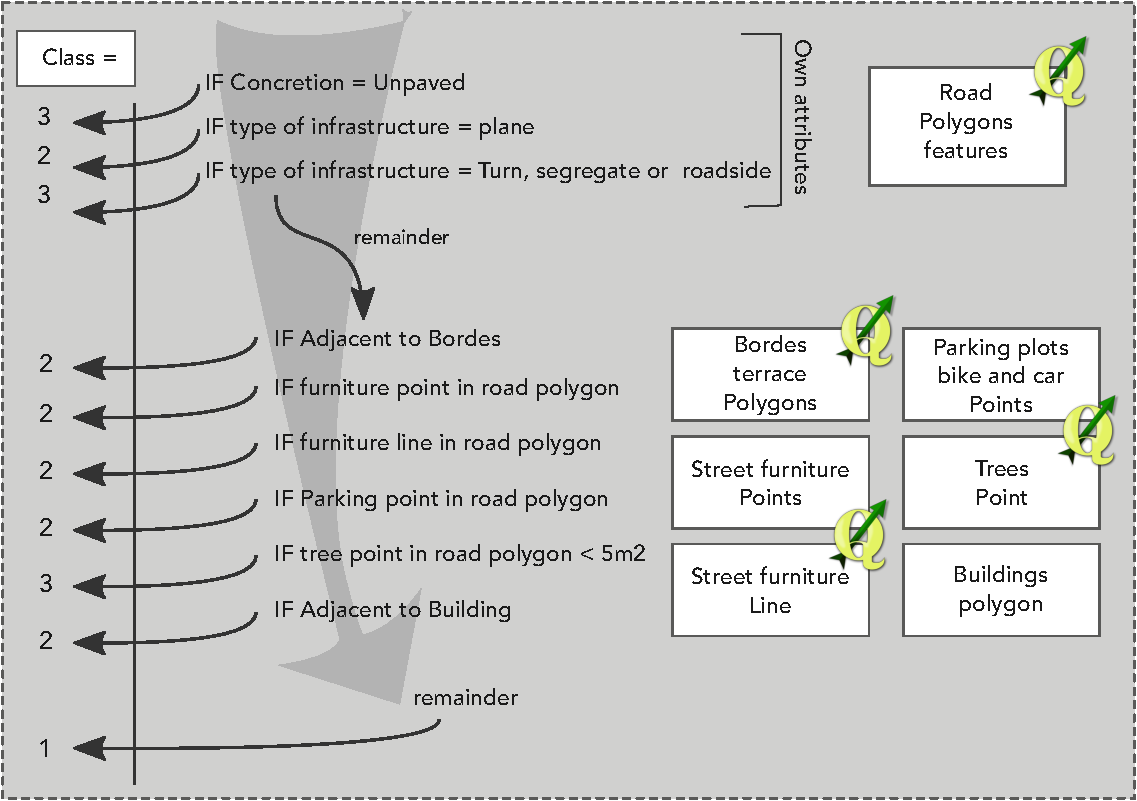
\includegraphics[width=\textwidth]{img/M_Pedestrianareaclassification.pdf}
\centering
\caption{ Classification steps road sections\label{classRoad}}
\end{figure}


\subsection{Data Collection and Pre-processing - AHN }
The AHN2 tiles covering the research area were downloaded from www.nationaalgeoregister.nl. The AHN is measured with laser altimetry or LIDAR. Laser beams shot from an air plane and localized with GPS. It is measured over several time periods and merged in the end to get a detailed measurement of the height. With a measured point density of 6 to 10 point per $m^2$~\cite{VanDerZon2013}. The eventual end product delivered is corrected to ground level, so vegetation, buildings and other object do not appear.~\cite{VanDerZon2013} These filtered areas are given no-data values. The raster data has a resolution of $0.5m^2$ and a precision of systematic and stochastic error of max $5cm$. The projection is the Dutch projected coordinate system RD new.~\cite{VanDerZon2013} Because the AHN2 is already delivered in RD new and corrected for ground level, no or little pre-processing is needed. Apart from downloading the correct tiles and merging these together for the appropriate area. 

\subsection{Analysis - Mapping sloping surfaces with AHN data}
The Policy of Amsterdam states that pedestrian areas with slopes more than 4\% is perceived negative.~\cite{leidraad2011}
The slope is derived from the AHN2. Also per road section, the average slope is calculated. The pedestrian classification with the GBKA are used to compare road sections for transport versus pedestrian area. 

\subsubsection{First derivative - Slope}
The first derivative or slope provides the degree of slope per pixel. This can be calculated with the following formula on cell to cell basis. 

\textbf{Degree of slope:}
\begin{equation}
\tan \theta = \frac{rise}{run}
\end{equation}
~\cite{ahnformula}

\textbf{So slope in degrees:}
\begin{equation}
\theta = \tanh \frac{\sqrt{\frac{dz}{dx}^2 + \frac{dz}{dy}^2 }*180 }{\pi}
\end{equation}
Source: ESRI 
http://webhelp.esri.com/arcgisdesktop/9.2/index.cfm?TopicName=How\%20Slope\%20works~\cite{ahnformula}


% \subsubsection{Second derivative - Curvature}
% Curvature is the second derivative of the surface, or the slope of the slope. Positive curvature is upward convex and negatives curvature is upward concave, at the cell. A value of 0 is a flat cell. The curvature of a surface is calculated on a cell-by-cell basis. For each cell, a fourth-order polynomial is calculated of the form:

% \begin{figure}[ht]
% 	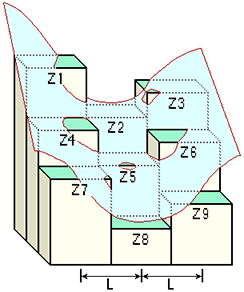
\includegraphics[width=0.25\textwidth]{img/M_curvature.png}
% 	\centering
% 	\caption{Curvature explained}
% 	\label{curvature}
% \end{figure}


% \begin{equation}
% Z = A_{x}^2 y^2 + B_{x}^2 y + C_{xy}^2 + D_{x}^2 + E_{y}^2 + F_{xy} + G_{x} + H_{y} + I
% \end{equation}
% Source ESRI:
% http:\slash\slash webhelp.esri.com \slash arcgisdesktop/ \slash9.2 \slashindex.cfm?TopicName=How\%20Curvature\%20works~\cite{ahnformula2}
% \slash